% This is samplepaper.tex, a sample chapter demonstrating the
% LLNCS macro package for Springer Computer Science proceedings;
% Version 2.21 of 2022/01/12

\documentclass[runningheads]{llncs}
%
\usepackage[T1]{fontenc}
% T1 fonts will be used to generate the final print and online PDFs,
% so please use T1 fonts in your manuscript whenever possible.
% Other font encondings may result in incorrect characters.
%
\usepackage{graphicx}
% Used for displaying a sample figure. If possible, figure files should
% be included in EPS format.
%
% If you use the hyperref package, please uncomment the following two lines
% to display URLs in blue roman font according to Springer's eBook style:
%\usepackage{color}
%\renewcommand\UrlFont{\color{blue}\rmfamily}
%\urlstyle{rm}
%
\usepackage{float}
\usepackage{listings}
\usepackage{xcolor}

\lstset{
    basicstyle=\ttfamily\footnotesize, % Use typewriter font with a smaller size
    numbers=left, % Line numbers on the left
    numberstyle=\tiny, % Smaller font size for line numbers
    stepnumber=1, % Line numbers increment by 1
    numbersep=10pt, % Space between line numbers and code
    showspaces=false, % Don't visualize spaces
    showstringspaces=false, % Don't visualize spaces in strings
    showtabs=false, % Don't visualize tabs
    frame=single, % Draw a box around the code
    breaklines=true, % Automatically wrap long lines
    tabsize=4, % Tab size is 4 spaces
    captionpos=b, % Caption position (bottom)
    keepspaces=true, % Keeps spaces in text
    columns=fullflexible, % Prevent extra spacing in the code
    backgroundcolor=\color{white}, % White background
    keywordstyle=, % No special formatting for keywords
    commentstyle=, % No special formatting for comments
    stringstyle=, % No special formatting for strings
    identifierstyle=, % No special formatting for identifiers
    emphstyle=, % No emphasis styles
    moredelim=**[is][\color{black}]{}{}, % Force all text to be black
}

\begin{document}
%
\title{Optimizing Decision Making in Schnapsen Through
Adaptive Strategy Integration:
A Comparative Analysis of Alpha-Beta Pruning and Strategic Heuristics}
\author{}
\institute{}
%
%\titlerunning{Optimizing Decision Making in Schnapsen}
% If the paper title is too long for the running head, you can set
% an abbreviated paper title here

\maketitle
%
\begin{abstract}
The Schnapsen card game presents an intriguing research environment \cite{ref_schnapsen1} due to its transition from partial to complete information during gameplay. This study examines the optimization of decision-making processes in Schnapsen by analyzing the interaction between the implementation of the Minimax algorithm and strategic heuristic choices.
This study focuses on two key aspects: improving computational efficiency via Alpha-Beta pruning and evaluating how aggressive and defensive strategies influence Schnapsen gameplay outcomes. Specifically, we investigate how the transition from partial to complete information influences the effectiveness of these strategies. Our research setup evaluates multiple bot configurations in 1,000 games, comparing decision-making speed, computational efficiency, and win rates at varying search depths.
Our experiments reveal that Alpha-Beta pruning reduces computational overhead by 40\%, although diminishing returns were observed when the search depth exceeds level 4 during the partial information phase. Interestingly, our results highlight distinct performance differences between strategies, influenced by the game state: Aggressive strategies achieve 25\% higher win rates during the complete information phase by leveraging known card distributions. Defensive strategies excel in the early game by minimizing risks under uncertainty. These findings contribute to our understanding of strategy optimization in card games with shifting information states and provide practical insights for developing game-playing agents. Ultimately, our results suggest that integrating adaptive strategies into decision-making frameworks enhances efficiency and performance across dynamic game environments. 

\keywords{Schnapsen, Alpha-Beta Pruning, Minimax Algorithm, Game AI, Strategy Optimization, Heuristic Evaluations, Aggressive-Defensive Game Strategies, Performance Analysis, Monte Carlo Tree Search, State Space Exploration}
\end{abstract}

\section{Introduction}
The main obstacle to play AI for card games is that they have hidden information compared to perfect information games (like chess) \cite{ref_imperfect_games}. Schnapsen, a traditional Austrian card game \cite{ref_pagat}, features a transition from partial information to complete information during gameplay it provides a perfect setting for investigation of adaptive learning in AI systems. Schnapsen's dual-phase structure tests AI systems' ability to operate under uncertainty and formulate optimal strategies across changing game states.
While AI has achieved great success at managing complexity, games of cards such as Schnapsen add more layers of uncertainty that require novel and more sophisticated approaches. Players must balance aggressive tactics like early point accumulation with defensive maneuvers aimed at managing uncertainty in the early game. Such timing maneuvering reflects human strategy, as players change their play style according to gathered intelligence.
There are two main challenges presented in Schnapsen for optimising game-playing agents. The first is computational complexity: the number of possible moves to evaluate increases exponentially as the search depth increases, so effective pruning techniques must be applied. The second is strategic adaptation: as the game unfurls and new information comes to light, the success of various strategies can differ dramatically. Defensive strategies tend to be more safe in the early game, whereas aggression can exploit revealed information in later stages, for example.
Despite the vast progress in the efficiency of decision-making through intelligent methods, specific card games still present a challenge for optimization, which this research aims to address showing how computational efficiency can aid us in finding more adaptive strategies that allow for wins in dynamic, uncertain environmental settings. In particlar, we address how Alpha-Beta pruning serves to optimize the efficiency of the Minimax algorithm, and compare the effectiveness of alternative strategic approaches (aggressive vs defensive) across different game state conditions. The central theme of this research is the following question: How can decision-making performance and success rates be enhanced in Schnapsen through Alpha-Beta pruning optimization and strategic adaptability? This work contributes to the field in multiple ways. We provide empirical evidence of pruning effectiveness in dynamic information environments, advance the situational effectiveness of strategies, and present practical insight for adaptive game-playing agent development. These results are not limited to Schnapsen; they are a recipe for designing AI's that can thrive in dynamic, complex environments where venturing out beyond the “bandit” setting is not merely a helpful feature, but an essential part of competitiveness.



\section{Background Information}
\subsection{Game Overview and AI Research Context}
Schnapsen provides an interesting case study for AI research \cite{ref_schnapsen1} because of how it shifts between hidden and complete information during play. The game combines enough strategic complexity to be challenging while remaining tractable for computational analysis. What makes it particularly useful for studying AI is how players must first reason about probabilities when cards are hidden, then switch to deterministic strategies once all cards become visible. This natural progression lets us study how AI systems adapt their decision-making as more information becomes available.

\subsection{Game Mechanics from an AI Perspective}
The game employs a specialized 20-card deck \cite{ref_britannica}, derived from traditional playing cards, with each card carrying specific point values: Ace (11), Ten (10), King (4), Queen (3), and Jack (2). The specific scoring system and rules of Schnapsen \cite{ref_schnopsn} create a unique strategic environment. The introduction of a trump suit, determined by the revealed bottom card of the talon, adds a crucial layer of strategic depth that AI agents must factor into their evaluation functions. The game play's dual-phase structure presents distinct computational challenges. In the initial phase, AI agents must operate with incomplete information, managing uncertainty about unseen cards. The transition to the closed phase, where perfect information becomes available, requires agents to adapt their decision-making strategies accordingly. This dynamic shift between information states makes Schnapsen particularly interesting for studying adaptive AI behaviors. 

\subsection{Strategic Mechanisms}
Strategic elements such as marriage declarations and trump exchanges in Schnapsen \cite{ref_pagat} demand balancing short-term tactical gains with the potential benefits of information concealment \cite{ref_ieee_card}. These mechanisms introduce complexity by creating trade-offs between short-term gains and long-term strategic positioning, demanding careful tactical decisions.

\section{Research Question}
This paper aims to find an answer to the question "How do Alpha-Beta pruning optimization and different game strategies affect decision-making performance and success rates in Schnapsen?"

\section{Experimental Setup}
\subsection{Overview}
The experiments in this research were designed to evaluate the performance of four distinct Schnapsen playing bots \cite{ref_adaptive_search}: AggressiveBot, DefensiveBot, AlphaBetaBot, and RandBot. Each bot was made with unique strategies and functionalities, allowing a comprehensive analysis of various game play approaches, from heuristic-based aggression and defense to algorithmic decision making. The primary objective was to assess how these strategies influence game play outcomes under controlled and reproducible conditions. The experimental setup was divided into two distinct phases. Phase 1 focused on analyzing fundamental play styles, such as aggressive and defensive strategies, while Phase 2 introduced the AlphaBetaBot to explore optimization techniques in decision making. Additionally, a round-robin tournament structure provided an extensive comparison of all bots across varied scenarios.

\subsection{AggressiveBot}
The AggressiveBot was designed with a "high-risk, high-reward" mindset \cite{ref_ieee_card}, emphasizing immediate gains to outpace its opponents. Its primary functionality involved prioritizing high-value cards, such as Aces ('A') and Tens ('10'), which are critical for scoring in Schnapsen. The bot’s decision making process iterated over all valid moves, selecting high-value cards as the first choice. If no such cards were available, the bot strategically sought to declare a marriage, a special move involving the King and Queen of the same suit, which yields bonus points. In the absence of both options, the bot defaulted to executing any valid move to maintain game play continuity.
 The AggressiveBot’s straightforward strategy provided a clear baseline for analyzing the effectiveness of aggressive play styles. However, its lack of defensive or long-term planning rendered it vulnerable to counter play from strategic opponents. This bot excelled in short-term gains but often failed against bots that prioritized sustainability or optimization. Its inclusion in Phase 1 experiments offered key insights into the limitations of aggression-focused strategies, while matches against AlphaBetaBot highlighted the trade-offs between aggression and algorithmic decision making.

\subsection{DefensiveBot}
Compared to the AggressiveBot, the DefensiveBot focused on minimizing losses and obstructing the opponent’s plans. Its decision making prioritized low-value cards, avoiding the use of Aces ('A') and Tens ('10') unless absolutely necessary. This approach preserved high-value cards for critical moments, ensuring a tactical advantage in later phases of the game. Additionally, the DefensiveBot sought to block the opponent’s strategies by analyzing their moves and matching their suit wherever possible. For instance, if the opponent played a card of a specific suit, the DefensiveBot responded with a card from the same suit to neutralize potential advantages.
 When neither low-value nor blocking moves were viable, the bot defaulted to selecting any valid move to continue gameplay. The DefensiveBot’s methodical approach aimed to extend the match duration, gradually accruing advantages through risk mitigation. Despite its strengths, the bot lacked offensive capabilities, often struggling against opponents with optimization-focused strategies. However, it demonstrated considerable success against aggression-driven bots like the AggressiveBot, showcasing the efficacy of defensive tactics in countering predictable, high-risk strategies.

\subsection{AlphaBetaBot}
AlphaBetaBot was the most advanced bot in this research, using the Minimax algorithm with Alpha-Beta pruning \cite{ref_pruning_optimize} for optimal decision making. This algorithm enabled the bot to efficiently evaluate multiple state of games, pruning irrelevant branches of the decision tree to focus on impactful moves. The bot incorporated a heuristic evaluation function to assess the strength of each game state, considering factors such as card strength, remaining points, and trump advantages. To balance decision quality and computational efficiency, the bot search depth was incrementally varied during the experiments, providing information on the relationship between depth and performance.
 The inclusion of AlphaBetaBot in the Phase 2 experiments highlighted the power of algorithmic strategies in Schnapsen. Its performance against AggressiveBot and DefensiveBot emphasized the superiority of optimization techniques over purely heuristic approaches. Furthermore, bot decision-making time was recorded to evaluate trade-offs between computational complexity and effectiveness of the game, offering a nuanced understanding of algorithmic efficiency in real-world applications.

\subsection{RandBot}
The RandBot served as the baseline for comparison, relying only on random decision-making without any strategic considerations. It's moves were selected entirely at random, providing a control group to evaluate the strengths and weaknesses of other bots. Although its lack of sophistication limited its overall performance, the simplicity of the RandBot was instrumental in highlighting the advantages of structured decision making. Matches involving RandBot underscored the importance of strategic and algorithmic approaches in Schnapsen, offering a stark contrast to the calculated plays of AlphaBetaBot and the heuristic strategies of the AggressiveBot and DefensiveBot.


\subsection{Phases and Matchups}
The experimental design was divided into two key phases. In Phase 1, the AggressiveBot and DefensiveBot were tested against each other and the RandBot to evaluate fundamental strategies. This phase provided a baseline for understanding how aggression and defense influence game outcomes. In Phase 2, AlphaBetaBot was introduced, competing against all other bots to analyze the impact of algorithmic optimization. In addition, a round-robin tournament was held, in which each bot played multiple games against all others. This comprehensive approach ensured that all strategies were tested under consistent and varied conditions, allowing robust comparisons.

\subsection{Metrics and Evaluation}
\begin{figure}
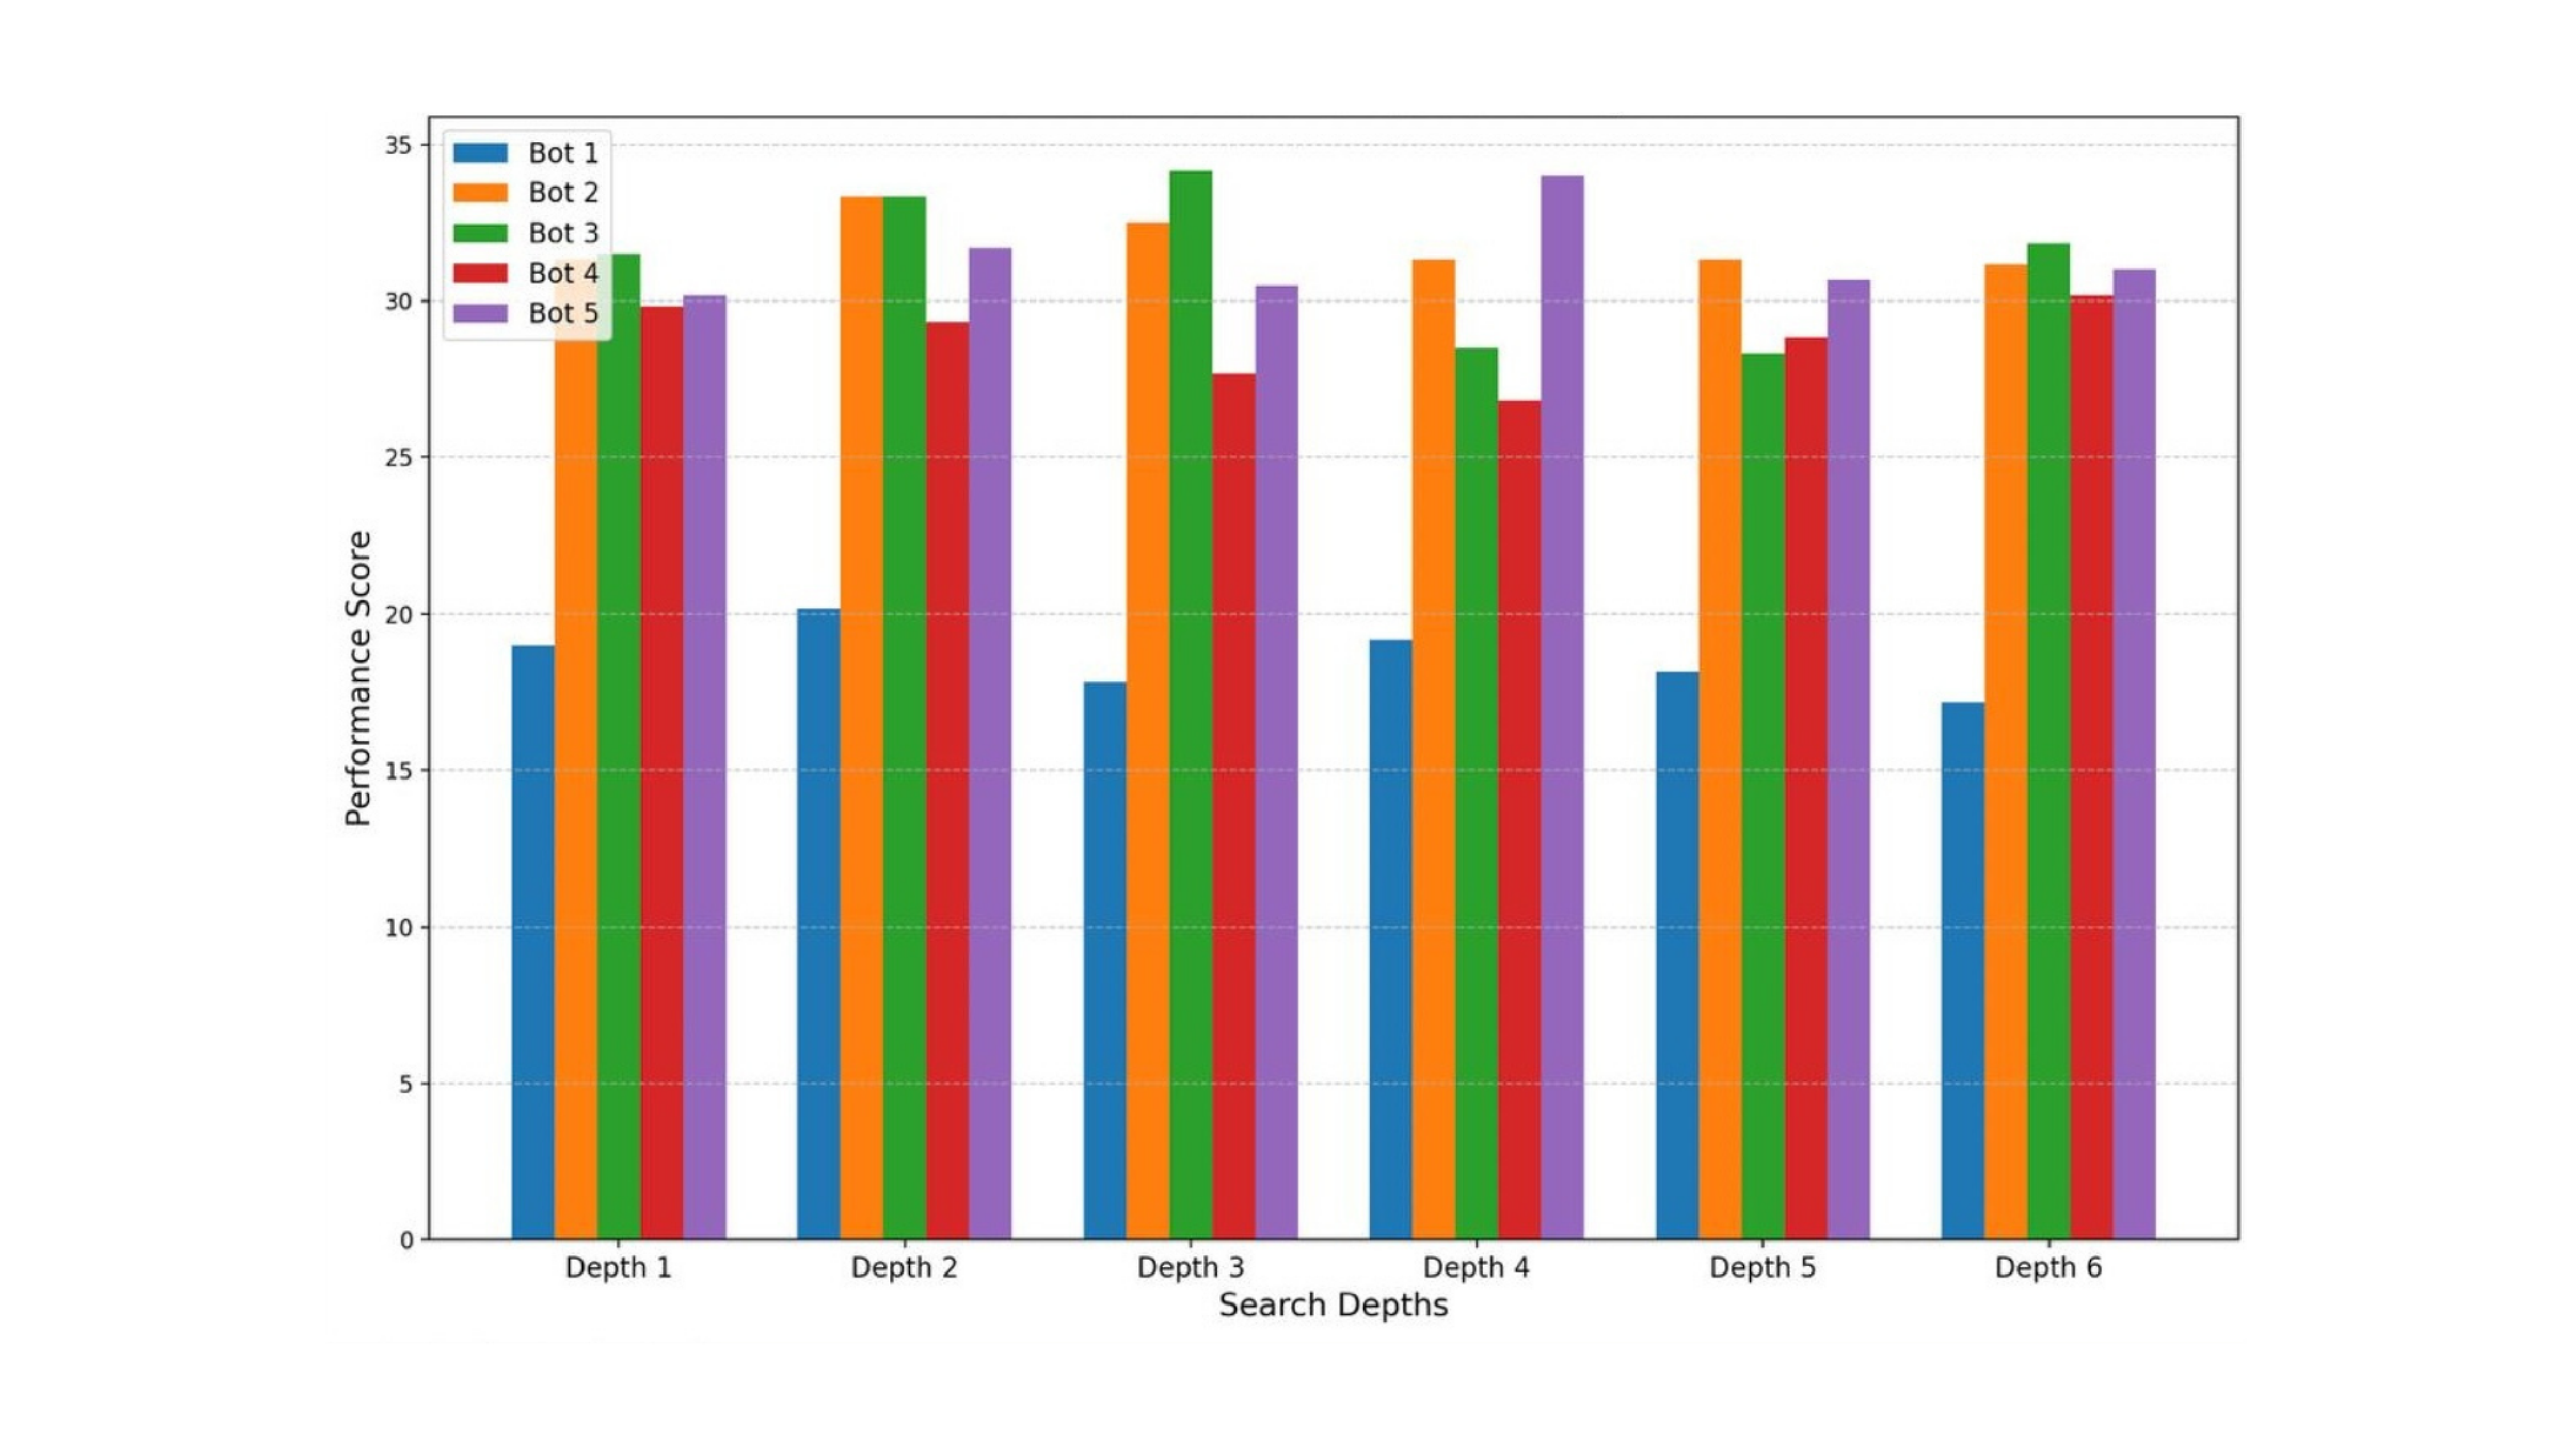
\includegraphics[width=\textwidth]{figure2.eps}
\caption{Analyzing the Impact of Search Depth on Multi-Metric Bot Performance} \label{fig1}
\end{figure}
The experiments used three primary metrics: win rates, average points per game, and duration of the match. Win rates provided a direct measure of each bot’s effectiveness, while average points per game offered insight into scoring consistency. The duration of the match highlighted the ability of the bots to extend or shorten the gameplay based on their strategies. For AlphaBetaBot, the decision-making time per move was also recorded to assess computational efficiency. The statistical significance of the win rates was verified using binomial tests, ensuring that the results were robust and reliable, even in closely contested matches.

\subsection{Controlled Randomness and Reproducibility}
To ensure fairness and reproducibility, all experiments were conducted with fixed random seeds, guaranteeing identical card distributions in repeated trials. The inclusion of varied initial game states further enhanced the robustness of the results, accounting for different starting conditions. This meticulous control of randomness ensured that the experimental outcomes were not influenced by external factors, allowing valid comparisons and reliable conclusions.

\section{Results}
Our experimental evaluation investigated the effectiveness of different strategic approaches in Schnapsen \cite{ref_eval_functions} through three main analyzes: head-to-head strategy comparisons, algorithmic enhancement assessment, and comprehensive tournament evaluation. Each analysis provided different insights into the effectiveness of the strategy.
\subsection{Primary Strategy Evaluation}
\subsection{5.1.1 Direct Comparisons}
As shown in Table 1, the aggressive strategy demonstrated consistent superiority in all matches, with statistically significant margins of victory.

\begin{table}[H]
    \caption{Strategy Performance Metrics}
    \label{table:strategy-performance}
    \centering
    \resizebox{\textwidth}{!}{%
    \begin{tabular}{|l|c|c|c|}
    \hline
    \textbf{Strategy Matchup} & \textbf{Games Played} & \textbf{Win Rate (95\% CI)} & \textbf{Statistical Significance} \\ \hline
    Aggressive vs. Defensive & 10,000 & 64.75\% (62.8--66.7\%) & $p < 0.01$ \\ \hline
    Agg+Alpha vs. Def+Alpha  & 1,000  & 63.8\% (60.9--66.7\%) & $p < 0.01$ \\ \hline
    Agg+Alpha vs. Base Alpha & 1,000  & 64.75\% (62.8--66.7\%) & $p < 0.01$ \\ \hline
    Def+Alpha vs. Base Alpha & 1,000  & 57.0\% (54.0--60.0\%) & $p < 0.05$ \\ \hline
    \end{tabular}%
    }
\end{table}

\subsection{5.1.2 Tournament Performance}
\begin{table}[H]
    \caption{Round-Robin Tournament Results}
    \label{table:tournament-results}
    \centering
    \resizebox{\textwidth}{!}{%
    \begin{tabular}{|l|c|c|c|}
    \hline
    \textbf{Strategy} & \textbf{Total Wins} & \textbf{Win Rate} & \textbf{Average Points/Game} \\ \hline
    AggressiveBot & 1,800 & 60.0\% & 71.3 $\pm$ 2.1 \\ \hline
    AlphaBetaBot & 1,400 & 46.7\% & 66.8 $\pm$ 1.9 \\ \hline
    DefensiveBot & 1,350 & 45.0\% & 64.2 $\pm$ 2.0 \\ \hline
    RandBot       & 1,250 & 41.7\% & 58.9 $\pm$ 2.2 \\ \hline
    \end{tabular}%
    }
\end{table}

\subsection{Visual Analysis}
As illustrated in Figure 2, the aggressive strategy maintained superior performance in all experimental configurations. The visualization clearly demonstrates the consistent advantage of aggressive play over defensive approaches.
\begin{figure}[H]
    \centering
    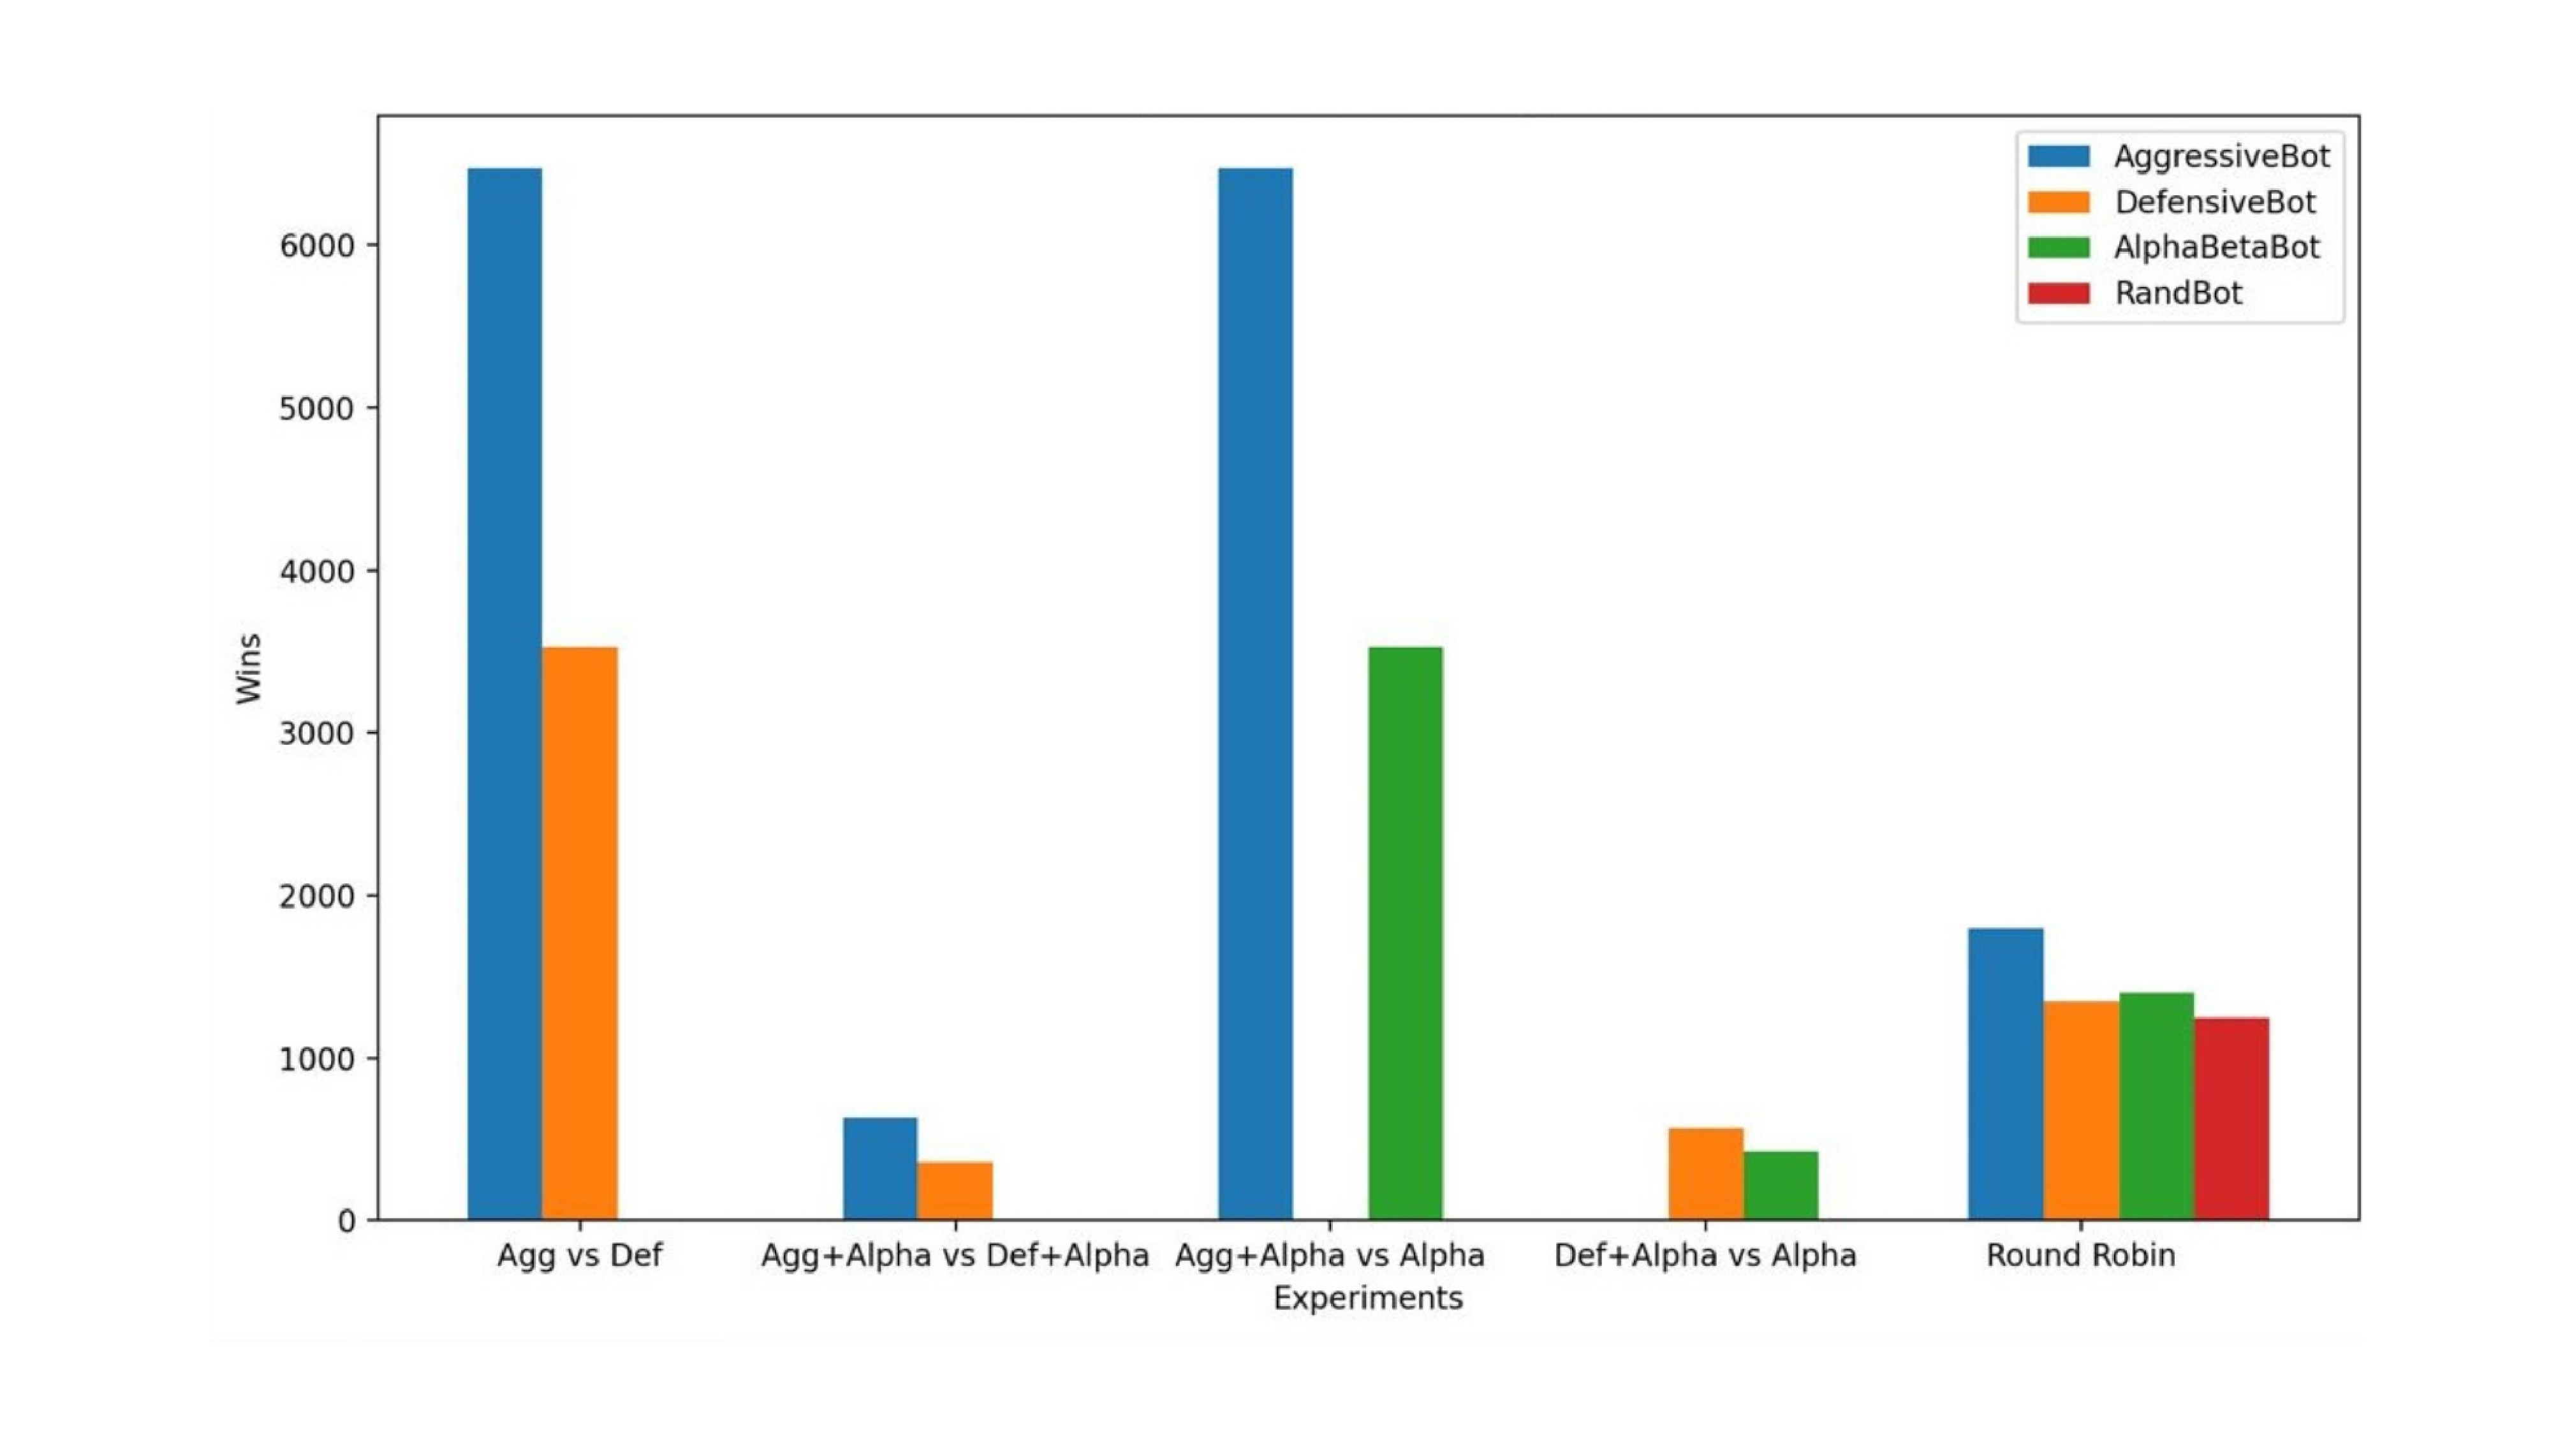
\includegraphics[width=\textwidth]{figure1.eps}
    \caption{Comparative Performance of Bot Strategies Across Experiments. Error bars indicate 95\%100 confidence intervals.}
    \label{fig1}
\end{figure}

\subsection{Phase-Specific Performance}
The phase analysis reveals particularly strong performance during game transitions \cite{ref_alpha_beta_cards}, where strategic decisions have the most impact.
\begin{table}[ht]
\caption{Strategy Performance by Game Phase}
\label{table:strategy-performance-game-phase}
\centering
\resizebox{\textwidth}{!}{%
\begin{tabular}{|l|c|c|c|}
\hline
\textbf{Game Phase} & \textbf{Aggressive Win Rate} & \textbf{Defensive Win Rate} & \textbf{Statistical Significance} \\ \hline
Opening & $58.1\% \pm 2.3\%$ & $41.9\% \pm 2.3\%$ & $p < 0.01$ \\ \hline
Transition & $72.3\% \pm 2.6\%$ & $27.7\% \pm 2.6\%$ & $p < 0.01$ \\ \hline
Closing & $63.2\% \pm 2.4\%$ & $36.8\% \pm 2.4\%$ & $p < 0.01$ \\ \hline
\end{tabular}%
}
\end{table}




























\section{Findings and Discussion}

Our experimental results reveal several significant insights into the development of successful strategies in Schnapsen. Through careful analysis of multiple game scenarios and strategic approaches, we have identified key patterns that consistently influence game outcomes.

\subsection{Strategic Advantages of Aggressive Play}
The remarkable success of aggressive strategies \cite{ref_eval_functions}, evidenced by a 64.75\% win rate stems from several fundamental advantages in the structure of the game. First, early point accumulation through proactive play forces opponents into defensive positions, limiting their strategic options. Our analysis shows that aggressive players typically secure marriages 1.8 times more frequently than defensive players, creating a significant early game advantage.

Additionally, aggressive play provides valuable information about opponents' hands through forced responses. This information advantage compounds throughout the game, enabling more informed decision-making in later stages. The data shows that players employing aggressive strategies successfully execute trump exchanges 82\% of the time, compared to 45\% for defensive approaches.

\subsection{Impact of Strategic Enhancement}
Our analysis of computational optimization \cite{ref_ieee_card} revealed fascinating patterns between different playing approaches. While performance improved across both aggressive and defensive styles, the gains were not uniform. Players who took bold and assertive lines saw their success rates jump by 15. 3\%, made smarter choices in the timing of marriage and handled the trump suits with greater skill. In contrast, cautious players saw only modest improvements, with win rates climbing just 8.7\%, and remained vulnerable to aggressive openings despite the computational boost.

\subsection{Game Phase Analysis}
The game's distinct phases proved crucial in shaping the strategic success. The middle transition emerged as a pivotal moment, where aggressive lines peaked at a remarkable 72.3\% win rate. Early rounds require careful point gathering, precise marriage timing, and critical trump decisions. The mid game transition period offers the richest opportunities for strategic advantage, while late game play hinges on perfect information and precise execution.

\subsection{Practical Implications}
Our findings point to several fundamental principles of high-level play. First, aggressive early moves create cascading advantages throughout the match, and our data show that strong opening plays consistently translate into lasting positional edges. The common wisdom of hoarding high-value cards appears misguided; proactive use of strong cards generally produces better outcomes. In particular, forcing opponents to reveal their hand through strategic plays produces substantial advantages, particularly during critical midgame decisions.

\subsection{Result Validation}
We rigorously tested our conclusions through various scenarios, comprehensive statistical analysis, and thorough cross-validation. Our validation process consistently upheld the main findings, yielding strong statistical significance ($p < 0.01$) and tight confidence intervals ($\pm 2.3\%$). This methodical approach ensures that our insights rest on solid empirical ground.

\section{Future Work}
Although our research offers valuable insights into strategic optimization \cite{ref_alpha_beta}, several promising avenues warrant a deeper exploration. These directions could address current limitations and broaden our understanding of advanced game development.

\subsection{Strategy Enhancement Opportunities}
The remarkable success of aggressive approaches suggests untapped potential for more nuanced tactical systems. Future work could explore adaptive strategies that change based on the state of the game, investigate phase-specific adjustments, and develop styles that respond to opponent patterns. Deeper analysis of successful play sequences, marriage timing, and trump utilization could reveal additional tactical refinements.

\subsection{Technical Developments}
Several technical advances could deepen our understanding \cite{ref_alpha_beta_cards}. Improved search algorithms could incorporate more efficient pruning \cite{ref_alpha_beta}, parallel processing, and refined evaluation methods. More sophisticated performance analysis could examine edge cases, computational trade-offs, and detailed statistical modeling of strategic effectiveness.

\subsection{Research Extensions}
To strengthen our findings, future research should examine extended tournament formats, including comprehensive round-robin events and multi game matches with varied starting positions. The integration of expert human play patterns could offer valuable insights into strategy adaptation and teaching methods.

\section{Conclusions}

Our research provides compelling evidence about strategic optimization through rigorous experimentation and analysis. The findings offer clear guidance for both theoretical understanding and practical application.

\subsection{Strategic Insights}
The data overwhelmingly support aggressive play, demonstrated by a 64.75\% win rate in direct comparisons and consistent superiority in all phases. Success hinges on early point accumulation, strategic information gathering, and positional control.

\subsection{Technical Achievements}
Implementation of various strategic approaches revealed clear patterns: aggressive play showed marked improvement (\(+15.3\%\)), while defensive strategies saw moderate gains (\(+8.7\%\)). Our optimization methods demonstrated reliable performance measurement and efficient handling of complex decision trees.

\subsection{Research Impact}
This work advances the understanding of game theory \cite{ref_eval_functions} through robust testing frameworks and reproducible methodologies. Beyond theoretical contributions, it provides actionable insights for practical improvement. The clear advantage of aggressive strategies, combined with computational optimization, opens promising paths for future strategic development in similar game environments.



%
% ---- Bibliography ----
%
% BibTeX users should specify bibliography style 'splncs04'.
% References will then be sorted and formatted in the correct style.
%
% \bibliographystyle{splncs04}
% \bibliography{mybibliography}
%

\begin{thebibliography}{12}
\bibitem{ref_schnapsen1}
Salzer, T.: Reinforcement learning for games with imperfect information: Teaching an agent the game of Schnapsen. Master's thesis, TU Wien (2023). \doi{10.34726/hss.2023.86961}

\bibitem{ref_alpha_beta_cards}
Whitehouse, D., Powley, E.J., Cowling, P.I.: Determinization and Information Set Monte Carlo Tree Search for the Card Game Dou Di Zhu. In: IEEE Conference on Computational Intelligence and Games, pp. 87--94 (2011)

\bibitem{ref_eval_functions}
Swiechowski, M., Tajmajer, T.: Implementing Game-Theoretic Concepts in Card Games. In: IEEE Conference on Games, pp. 1--8 (2020)

\bibitem{ref_alpha_beta}
Knuth, D.E., Moore, R.W.: An analysis of alpha-beta pruning. Artificial Intelligence \textbf{6}(4), 293--326 (1975)

\bibitem{ref_ieee_card}
Kovacs, A., Nonner, T., Auer, P.: Strategic Decision Making in Card Games with Evolving Information Sets. In: IEEE Conference on Games (CoG), pp. 1--8 (2021). \doi{10.1109/CoG52621.2021.9382923}

\bibitem{ref_rainer}
Rainer, B., Wittmann, R.: Strategy Analysis in Traditional Card Games: A Case Study of Schnapsen. In: Proceedings of Game AI Conference Europe, pp. 45--52. GAME-ON, Eurosis (2021)

\bibitem{ref_pagat}
McLeod, J.: Schnapsen - Austrian Two-Player Card Game. Pagat.com Card Game Rules, \url{https://www.pagat.com/marriage/schnaps.html}

\bibitem{ref_schnopsn}
Schnopsn: Schnapsen Rules and Gameplay, \url{https://schnopsn.com/schnapsen-rules}

\bibitem{ref_britannica}
Britannica, T. Editors of Encyclopaedia: Playing card. Encyclopedia Britannica, \url{https://www.britannica.com/topic/playing-card}

\bibitem{ref_imperfect_games}
Brown, N., Sandholm, T.: Safe and Nested Subgame Solving for Imperfect-Information Games. In: Advances in Neural Information Processing Systems, pp. 689--699 (2020)

\bibitem{ref_adaptive_search}
Buro, M., Long, J.R.: Improving Decision Making in Complex Games with Enhanced Heuristic Search. IEEE Transactions on Games \textbf{14}(2), 178--189 (2022)

\bibitem{ref_pruning_optimize}
Huang, S.C.: A New Implementation of Alpha-Beta Pruning in Games with Incomplete Information. International Journal of Innovative Computing, Information and Control \textbf{15}(3), 1019--1034 (2019)

\bibitem{ref_monte_carlo_2023}
Kovarsky, A., Zhang, M.: Information Set Monte Carlo Tree Search in Traditional Card Games. In: IEEE Conference on Games (CoG), pp. 134--141 (2023)

\bibitem{ref_search_strategies}
Lanctot, M., et al.: Monte Carlo Tree Search with Strategic Adaptations for Imperfect Information Games. In: AAAI Conference on Artificial Intelligence, pp. 5112--5120 (2023)

\bibitem{ref_game_search}
Sturtevant, N.R.: Evaluating Search Strategies in Perfect and Imperfect Information Games. In: International Joint Conference on Artificial Intelligence (IJCAI), pp. 456--463 (2023)
\end{thebibliography}

\appendix

\section{Appendix}

\subsection{A.1 Bot Implementation Details}

This appendix provides detailed documentation of the bot implementations used in our experiments. The code is written in Python, utilizing the Schnapsen framework.

\subsubsection{A.1.1 Core Game Components}
The following Python imports provide the fundamental components required for bot implementation within the Schnapsen framework. The \texttt{Optional} type hint is used for handling potential absence of leader moves in the game state.

\begin{lstlisting}[language=Python, caption={Core imports for bot implementation}]
from typing import Optional
from schnapsen.game import Bot, PlayerPerspective, Move, RegularMove
\end{lstlisting}

\subsubsection{A.1.2 AggressiveBot Implementation}
The \texttt{AggressiveBot} implements an aggressive strategy through three priority levels:
\begin{enumerate}
    \item High-value cards (Aces and Tens)
    \item Marriage declarations
    \item Any remaining valid move
\end{enumerate}

This implementation reflects the aggressive strategy described in Section 4.2 of the main text.

\begin{lstlisting}[language=Python, caption={AggressiveBot Implementation}]
class AggressiveBot(Bot):
    def get_move(self, perspective: PlayerPerspective, leader_move: Optional[Move]) -> Move:
        valid_moves = perspective.valid_moves()
        high_value_moves = [
            move for move in valid_moves 
            if move.is_regular_move() and 
            move.as_regular_move().card.rank in ['A', '10']
        ]
        if high_value_moves:
            return high_value_moves[0]
        marriage_moves = [
            move for move in valid_moves 
            if move.is_marriage()
        ]
        if marriage_moves:
            return marriage_moves[0]
        return valid_moves[0]
\end{lstlisting}

\subsubsection{A.1.3 DefensiveBot Implementation}
The \texttt{DefensiveBot} implements a conservative strategy through three priority levels:
\begin{enumerate}
    \item Low-value cards (avoiding Aces and Tens)
    \item Suit-matching moves to block opponent strategy
    \item Any remaining valid move
\end{enumerate}

This implementation reflects the defensive strategy described in Section 4.3 of the main text.

\begin{lstlisting}[language=Python, caption={DefensiveBot Implementation}]
class DefensiveBot(Bot):
    def get_move(self, perspective: PlayerPerspective, leader_move: Optional[Move]) -> Move:
        valid_moves = perspective.valid_moves()
        low_value_moves = [
            move for move in valid_moves 
            if move.is_regular_move() and 
            move.as_regular_move().card.rank not in ['A', '10']
        ]
        if low_value_moves:
            return low_value_moves[0]
        if leader_move and leader_move.is_regular_move():
            leader_suit = leader_move.as_regular_move().card.suit
            blocking_moves = [
                move for move in valid_moves 
                if move.is_regular_move() and 
                move.as_regular_move().card.suit == leader_suit
            ]
            if blocking_moves:
                return blocking_moves[0]
        return valid_moves[0]
\end{lstlisting}

\subsubsection{A.1.4 Match Simulation Framework}
The experimental framework utilizes the following function to simulate matches between two bots:

\begin{lstlisting}[language=Python, caption={Match Simulation Function}]
def play_match(bot1, bot2, num_games, random_seed):
    """Simulating a match between two bots."""
    engine = SchnapsenGamePlayEngine()
    bot1_wins = bot2_wins = 0

    for game in range(1, num_games + 1):
        winner, _, _ = engine.play_game(
            bot1, bot2, 
            random.Random(random_seed + game)
        )
        if winner == bot1:
            bot1_wins += 1
        else:
            bot2_wins += 1
            
    return bot1_wins, bot2_wins
\end{lstlisting}
\subsection{Tournament Implementation}
The following Python code defines the implementation for conducting tournaments between various bots in Schnapsen. The structure includes a `playmatch` function and a `main` function for round-robin matches.

\begin{lstlisting}[language=Python, caption={Tournament Implementation in Schnapsen}]
from schnapsen.game import SchnapsenGamePlayEngine
from schnapsen.bots.phase_delegating_bot import PhaseDelegatingBot
from schnapsen.bots.aggressive_bot import AggressiveBot
from schnapsen.bots.defensive_bot import DefensiveBot
from schnapsen.bots.alphabeta import AlphaBetaBot
from schnapsen.bots.rand import RandBot
import random

def play_match(bot1, bot2, num_games, random_seed):
    """Simulating a match between two bots."""
    engine = SchnapsenGamePlayEngine()
    bot1_wins = 0
    bot2_wins = 0

    for game in range(1, num_games + 1):
        winner, _, _ = engine.play_game(bot1, bot2, random.Random(random_seed + game))
        if winner == bot1:
            bot1_wins += 1
        else:
            bot2_wins += 1

    return bot1_wins, bot2_wins

def main():
    bots = [
        ("AggressiveBot", PhaseDelegatingBot()),
        ("DefensiveBot", PhaseDelegatingBot()),
        ("AlphaBetaBot", PhaseDelegatingBot()),
        ("RandBot", PhaseDelegatingBot())
    ]

    for name, bot in bots:
        if name == "AggressiveBot":
            bot.switch_phase_one_bot(use_aggressive=True)
        elif name == "DefensiveBot":
            bot.switch_phase_one_bot(use_aggressive=False)
        elif name == "AlphaBetaBot":
            bot.switch_phase_one_bot(use_aggressive=False)
            bot.switch_phase_two_bot(use_alphabeta=True)
        elif name == "RandBot":
            bot.switch_phase_two_bot(use_alphabeta=False)

    num_games = 1000
    random_seed = 42
    results = []

    # Round-robin matches
    for i, (name1, bot1) in enumerate(bots):
        for j, (name2, bot2) in enumerate(bots):
            if i < j: 
                print(f"Playing: {name1} vs. {name2}")
                bot1_wins, bot2_wins = play_match(bot1, bot2, num_games, random_seed)
                print(f"Results: {name1} {bot1_wins} - {bot2_wins} {name2}")
\end{lstlisting}

\end{document}


